
%%%%%%%%%%%%%%%%%%%%% Results %%%%%%%%%%%%%%%%%%%%%%%%%%%%%%%%%

\section{Results}


\subsection{Gene mutations and IGHV are main drivers of gene expression variability in CLL} 
Previous studies found a limited impact of known disease subgroups on GEP \citep{ Rosenwald2001}. To obtain an overview of  drivers for gene expression variability in CLL, we performed hierarchical clustering based on the 1000 most variable genes (figure \ref {fig:data_overview}A). Hierarchical clustering showed a clear separation of distinct subgroups which segregated with IGHV, methylation status and presence of trisomy 12.  These results were supported by principal component analysis (PCA)(figure \ref {fig:data_overview}C) and suggest that genetic subgroups in CLL shape gene expression to a previously underappreciated extend. We found PC1, which represented $9.5 \%$ of variance, to be associated with IGHV status and PC2 and PC3 separated samples based on trisomy 12. Besides these main drivers, we also found numerous differentially expressed genes associated with further genetic variants including SF3B1, BRAF, NOTCH1 and TP53 mutation (figure \ref {fig:data_overview}B).\\

A large  previous gene expression study in CLL described c1/c2 groups, which were found to be associated with B cell receptor activation and outcome \citep{Ferreira2014a}. We used hierarchical clustering with the differentially expressed genes characteristic of c1/c2, which indeed revealed two main clusters. In our data set, these differentially expressed genes showed very low variability across samples . In addition, none of PC1 - PC10 showed associations to the c1/2 subgroups and we could not identify an association of C1/C2 with outcome including time to next treatment or survival (data not shown). Recent data suggested the process associated with C1/2 gene expression being related to transcriptional changes linked to blood collection procedures and nonsense mediated decay \citep{Dvinge2014}. In our analysis gene expression changes associated with C1/C2 add little variance compared to other sources of variability.  

%----------------------------------------------------------------------------------------------------
% Fig.1: The effects of IGHV status, tumor mutations and DNA methylation status on gene expression
%----------------------------------------------------------------------------------------------------
\begin{figure}
	\centering
	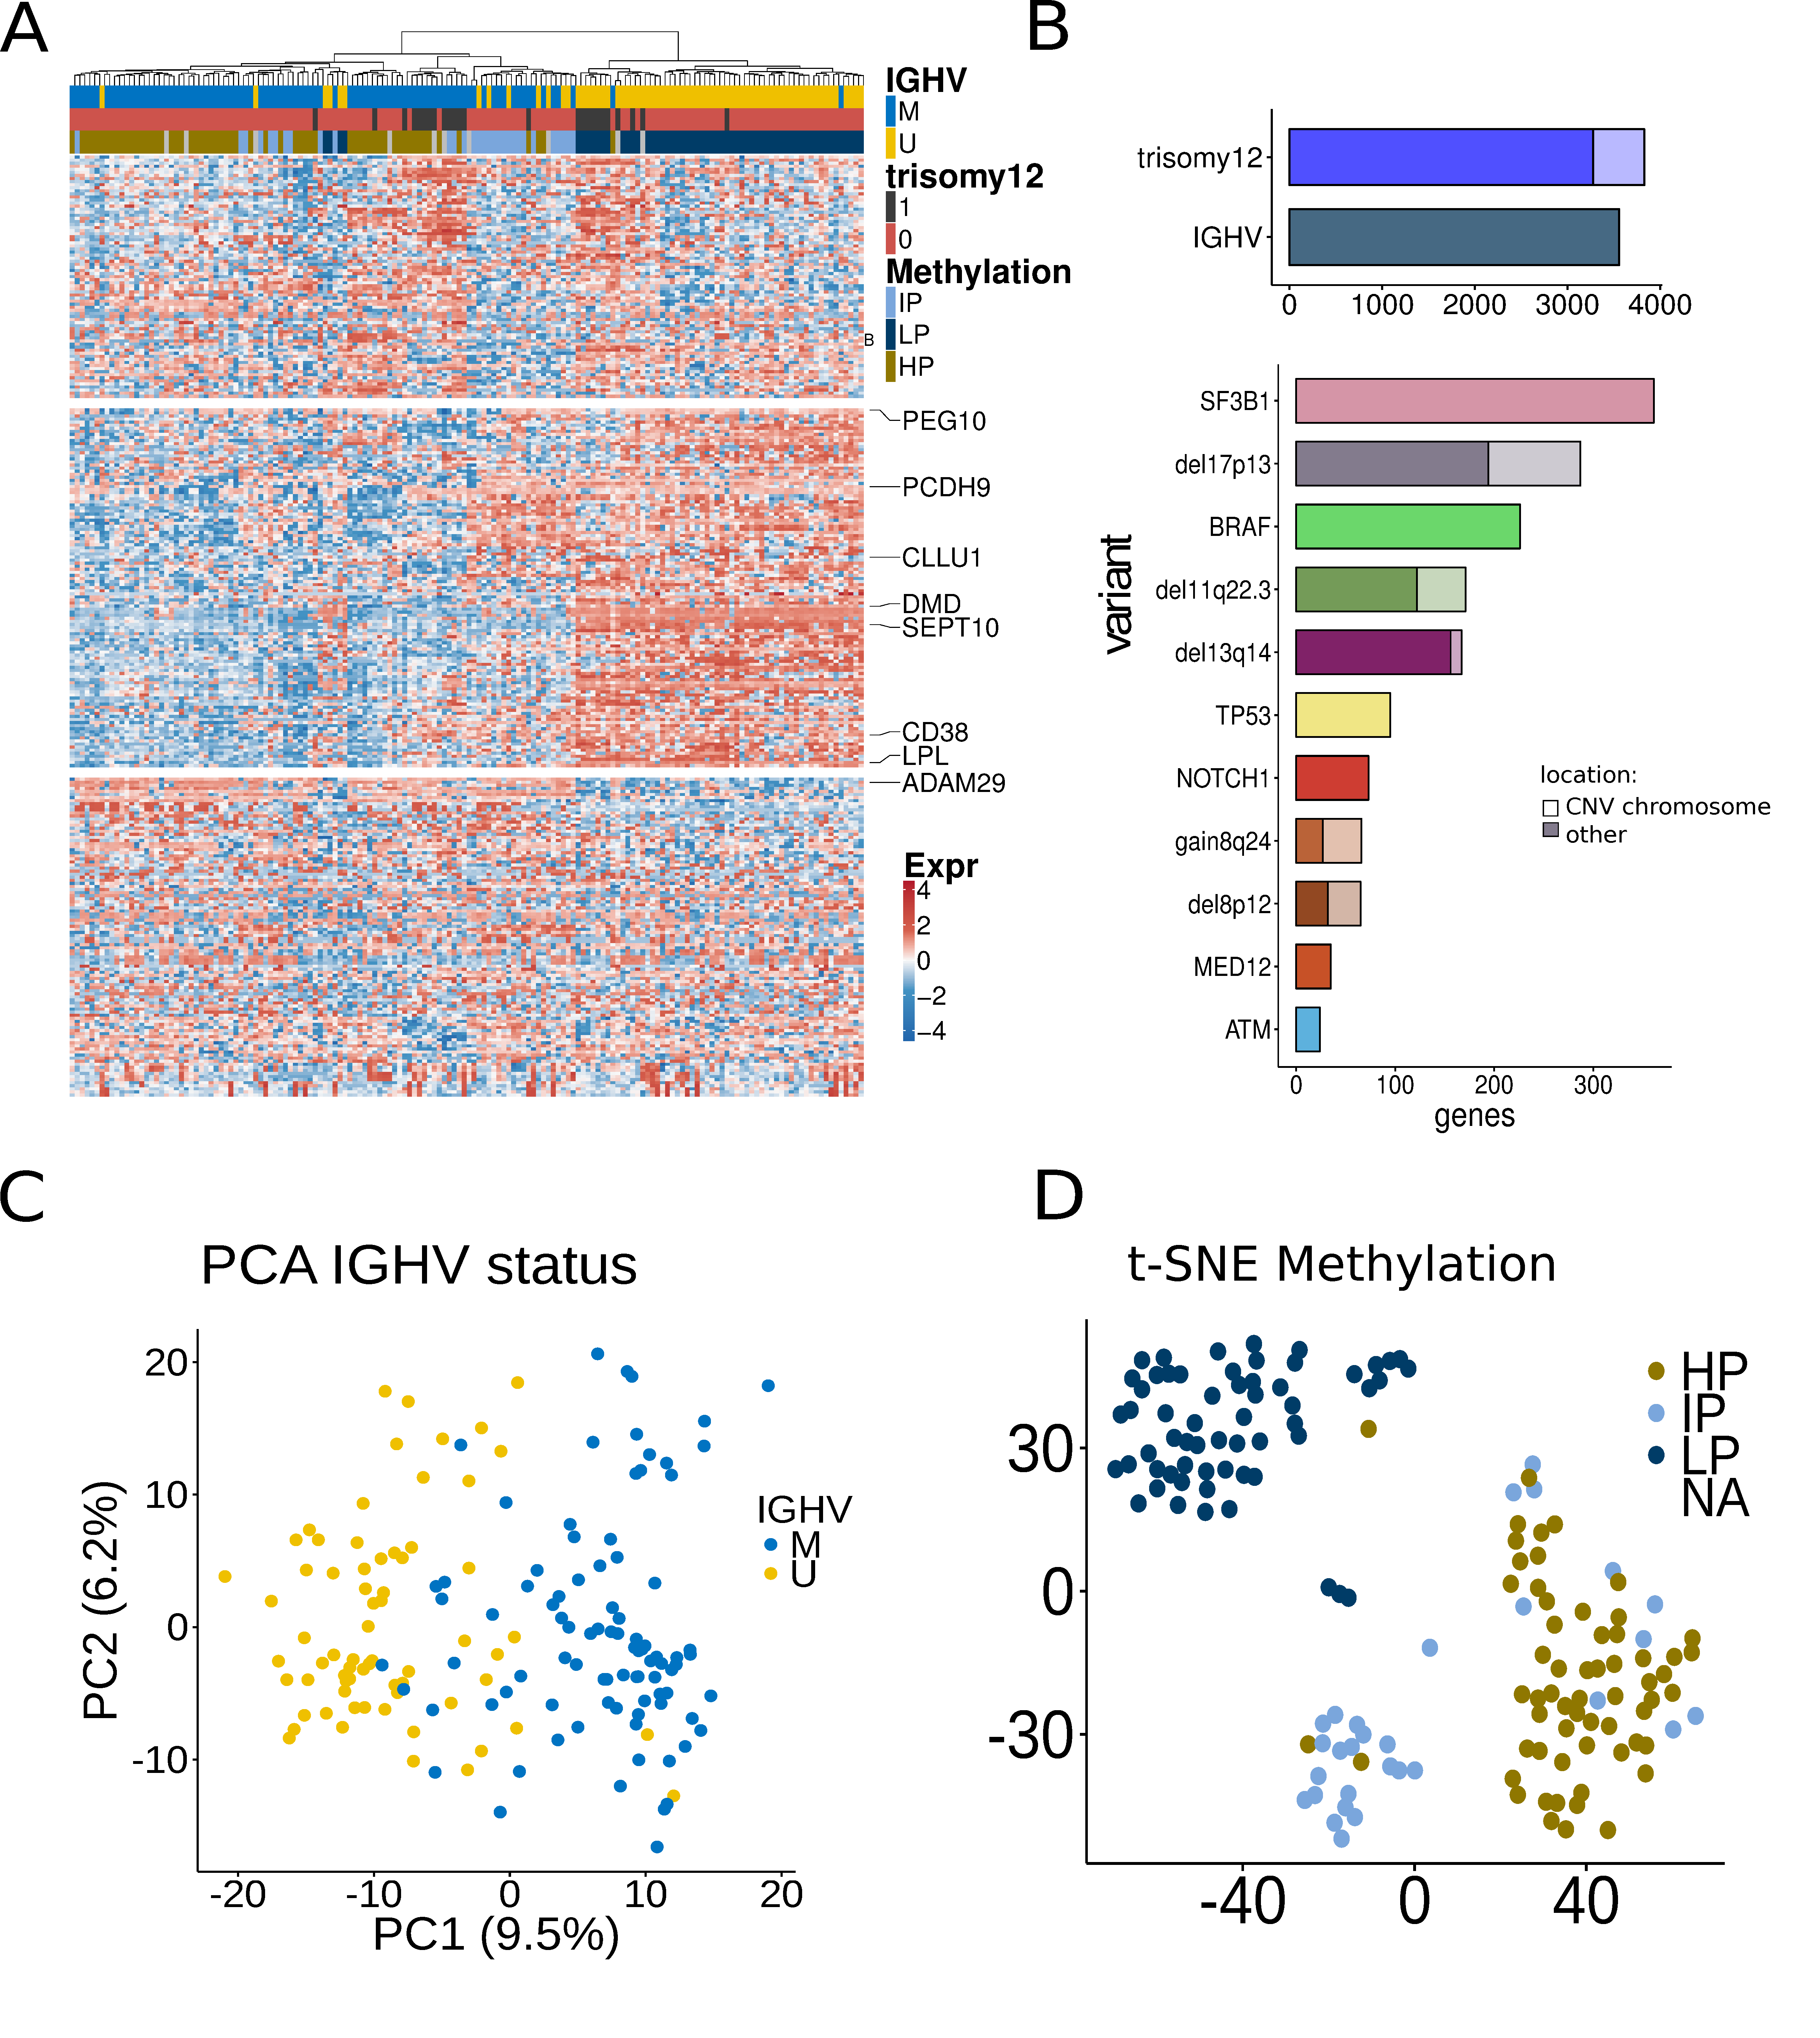
\includegraphics[width=\columnwidth]{figures/data_overview_geneCluster_new.pdf}
	\caption{\textbf{Gene expression variability in CLL:} A) Hierarchical clustering of CLL samples based on the 1000 most variable genes. IGHV groups and Trisomy12 samples form major cluster. B) Number of differentially expressed genes ($\text{p}_\text{adj} < 0.01$) for genomic markers. C) IGHV status is associated with the 1st principal component, which explains 9.5\% of variance. D) Two-dimensional $t$-distributed stochastic neighbour embedding ($t$-SNE) plot, based on sample distances using the 150 most variable genes. Distinct clusters are associated with the DNA methylation groups.}
	\label{fig:data_overview}
\end{figure}

\clearpage

\subsubsection{IGHV status is linked to distinct expression changes} 

To assess the influence of genetic drivers on gene expression in detail, we analysed gene expression changes for the most prevalent mutations and copy number variants of CLL. The somatic hypermutation status of IGHV was a main determinant of gene expression variability.  We found 3275 genes significantly differentially expressed between M-CLL and U-CLL after adjustment for multiple testing using the method of Benjamini and Hochberg for FDR = 1\%(figure \ref {fig:data_overview}B). In total 9.5 \% of variance within gene expression was associated with the IGHV status (figure \ref {fig:data_overview}C). This revealed a larger impact on transcriptional changes than previously detected \citep{Ferreira2014a}. Genes previously found to be good markers related to the IGHV status include CD38, LPL, ZAP70, SEPT10, ADAM29 and PEG10 \citep{Kienle2010}, and were also associated with IGHV in our study (figure \ref {fig:IGHV_expression}A/D). Besides this, we identified new marker genes associated with IGHV as PTCH1 and FGFR1 (figure \ref {fig:IGHV_expression}D). PTCH1 is a Hedgehog signalling pathway component and was associated with CLL before \citep{Decker2012}. The fibroblast growth factor receptor FGFR1 is related to cell growth and survival and is studied as potential target in the context of several other cancer types \citep{Zhou2016}. Different IGHV genes were also found among the most differentially expressed genes, but showed heterogenous expression within the U and M-CLL groups. Commonly used IGHV Receptors (1-69 or 4-34) associated with U and M-CLL, respectively. We compared IGHV1-69 gene expression with data from IG gene analysis in the corresponding samples. Gene expression showed a strong relation to IG gene usage (figure \ref {fig:IGHV_expression}B) and these data suggest, that RNA sequencing can be used to assess IG gene usage. \\

To understand pathways involved in U- and M-CLL we performed gene set enrichment analysis. Differentially expressed genes between IGHV genes were enriched in B cell receptor signalling, T cell receptor signalling as well as in ribosomal genes, several cancer pathways and chemokine signalling pathways (figure \ref {fig:IGHV_expression}C). Detailed summaries of the deregulated genes within these pathways are shown in the supplements (Supplement figure \ref {fig:IGHV_expression}). \\ 

Within the B cell receptor signalling gene set we identified cell surface molecules (CD19, CD22, CD81) and NFAT and NFkB signalling pathways to be downregulated. 
From the “T cell receptor signalling” gene set, ZAP70, PAK and p38 were upregulated in U-CLL, while IL10 and SHP1 were downregulated.
For chemokine signalling pathways, we found downregulation of CXCR3 and CXCR4 in U-CLL, while a set of Interferons (IFNB1, INFA21) were upregulated. \\

In summary our data are in line with the major biological role of IGHV mutation status in CLL and provide a rich resource to assemble deregulated pathways in the disease.



\begin{figure}
	\centering
	\includegraphics[width=\columnwidth]{figures/gene_summary_IGHV.pdf}
	\caption{\textbf{Gene expression changes between IGHV groups:} A)Differentially expressed genes between IGHV groups with $\text{p}_\text{adj} < 0.01$, $\log_2$ fold change $>2$ and basemean $> 500$. B) IGHV1-69 expression by corresponding IGHV1-69 variant usage determined in IG gene analysis. C) Enriched pathways between IGHV groups. D) Normalized gene counts for FGFR1, ZAP70 and PTCH1 separated by IGHV status.}
	\label{fig:IGHV_expression}
\end{figure}

\clearpage

\subsubsection{Trisomy12 expression signature}
We identified 3557 differentially expressed genes with $\text{p}_\text{adj} < 0.01$ in trisomy12 samples. To narrow them down, we filtered them by $\log_2$ fold change $>2$ and basemean $> 500$. The basemean describes the mean of normalized counts of all samples, normalizing for sequencing depth \citep{Love2014}. We find distinct expression pattern of up- and downregulated genes for  trisomy 12 samples (see figure \ref {fig:trisomy12}A). Even though many upregulated genes are located on chromosome 12, the majority of differentially expressed genes are distributed among the other chromosomes and can not be ascribed to a dosage effect (see figure \ref {fig:trisomy12}A,B). Among differentially expressed genes we found numerous marker of integrin signalling as SOCS3, ITGB2-AS1 and RAPGEF5. In addition endocytosis is one of the enriched pathways in trisomy12 (see table \ref {tabular:summary}) and we find genes coding for adhesion molecules like GIT2 and ADD2 up regulated. This is in line with previous findings about increased lymph node homing via cellular adhesion and transendothelial migration of circulating cells into the lymph node in trisomy12 \citep{Riches2014,Ganghammer2015}. We also find important checkpoint genes like the immune checkpoint CTLA4  and the cell cycle regulator CHFR differentially expressed in trisomy12. Both are associated with increased proliferation and tumor progression \citep{Mittal2013, Oh2009} and reveal mechanisms used by trisomy12 to promote tumor growth. Altogether these results suggest that modulation of the microenviroment and deregulation of cell cycle checkpoint genes are important mechanism in trisomy12 tumorigenesis. 

%----------------------------------------------------------------------------------------------------
% Fig.2: Gene expression signature of trisomy12
%----------------------------------------------------------------------------------------------------

\begin{figure}
	\centering
	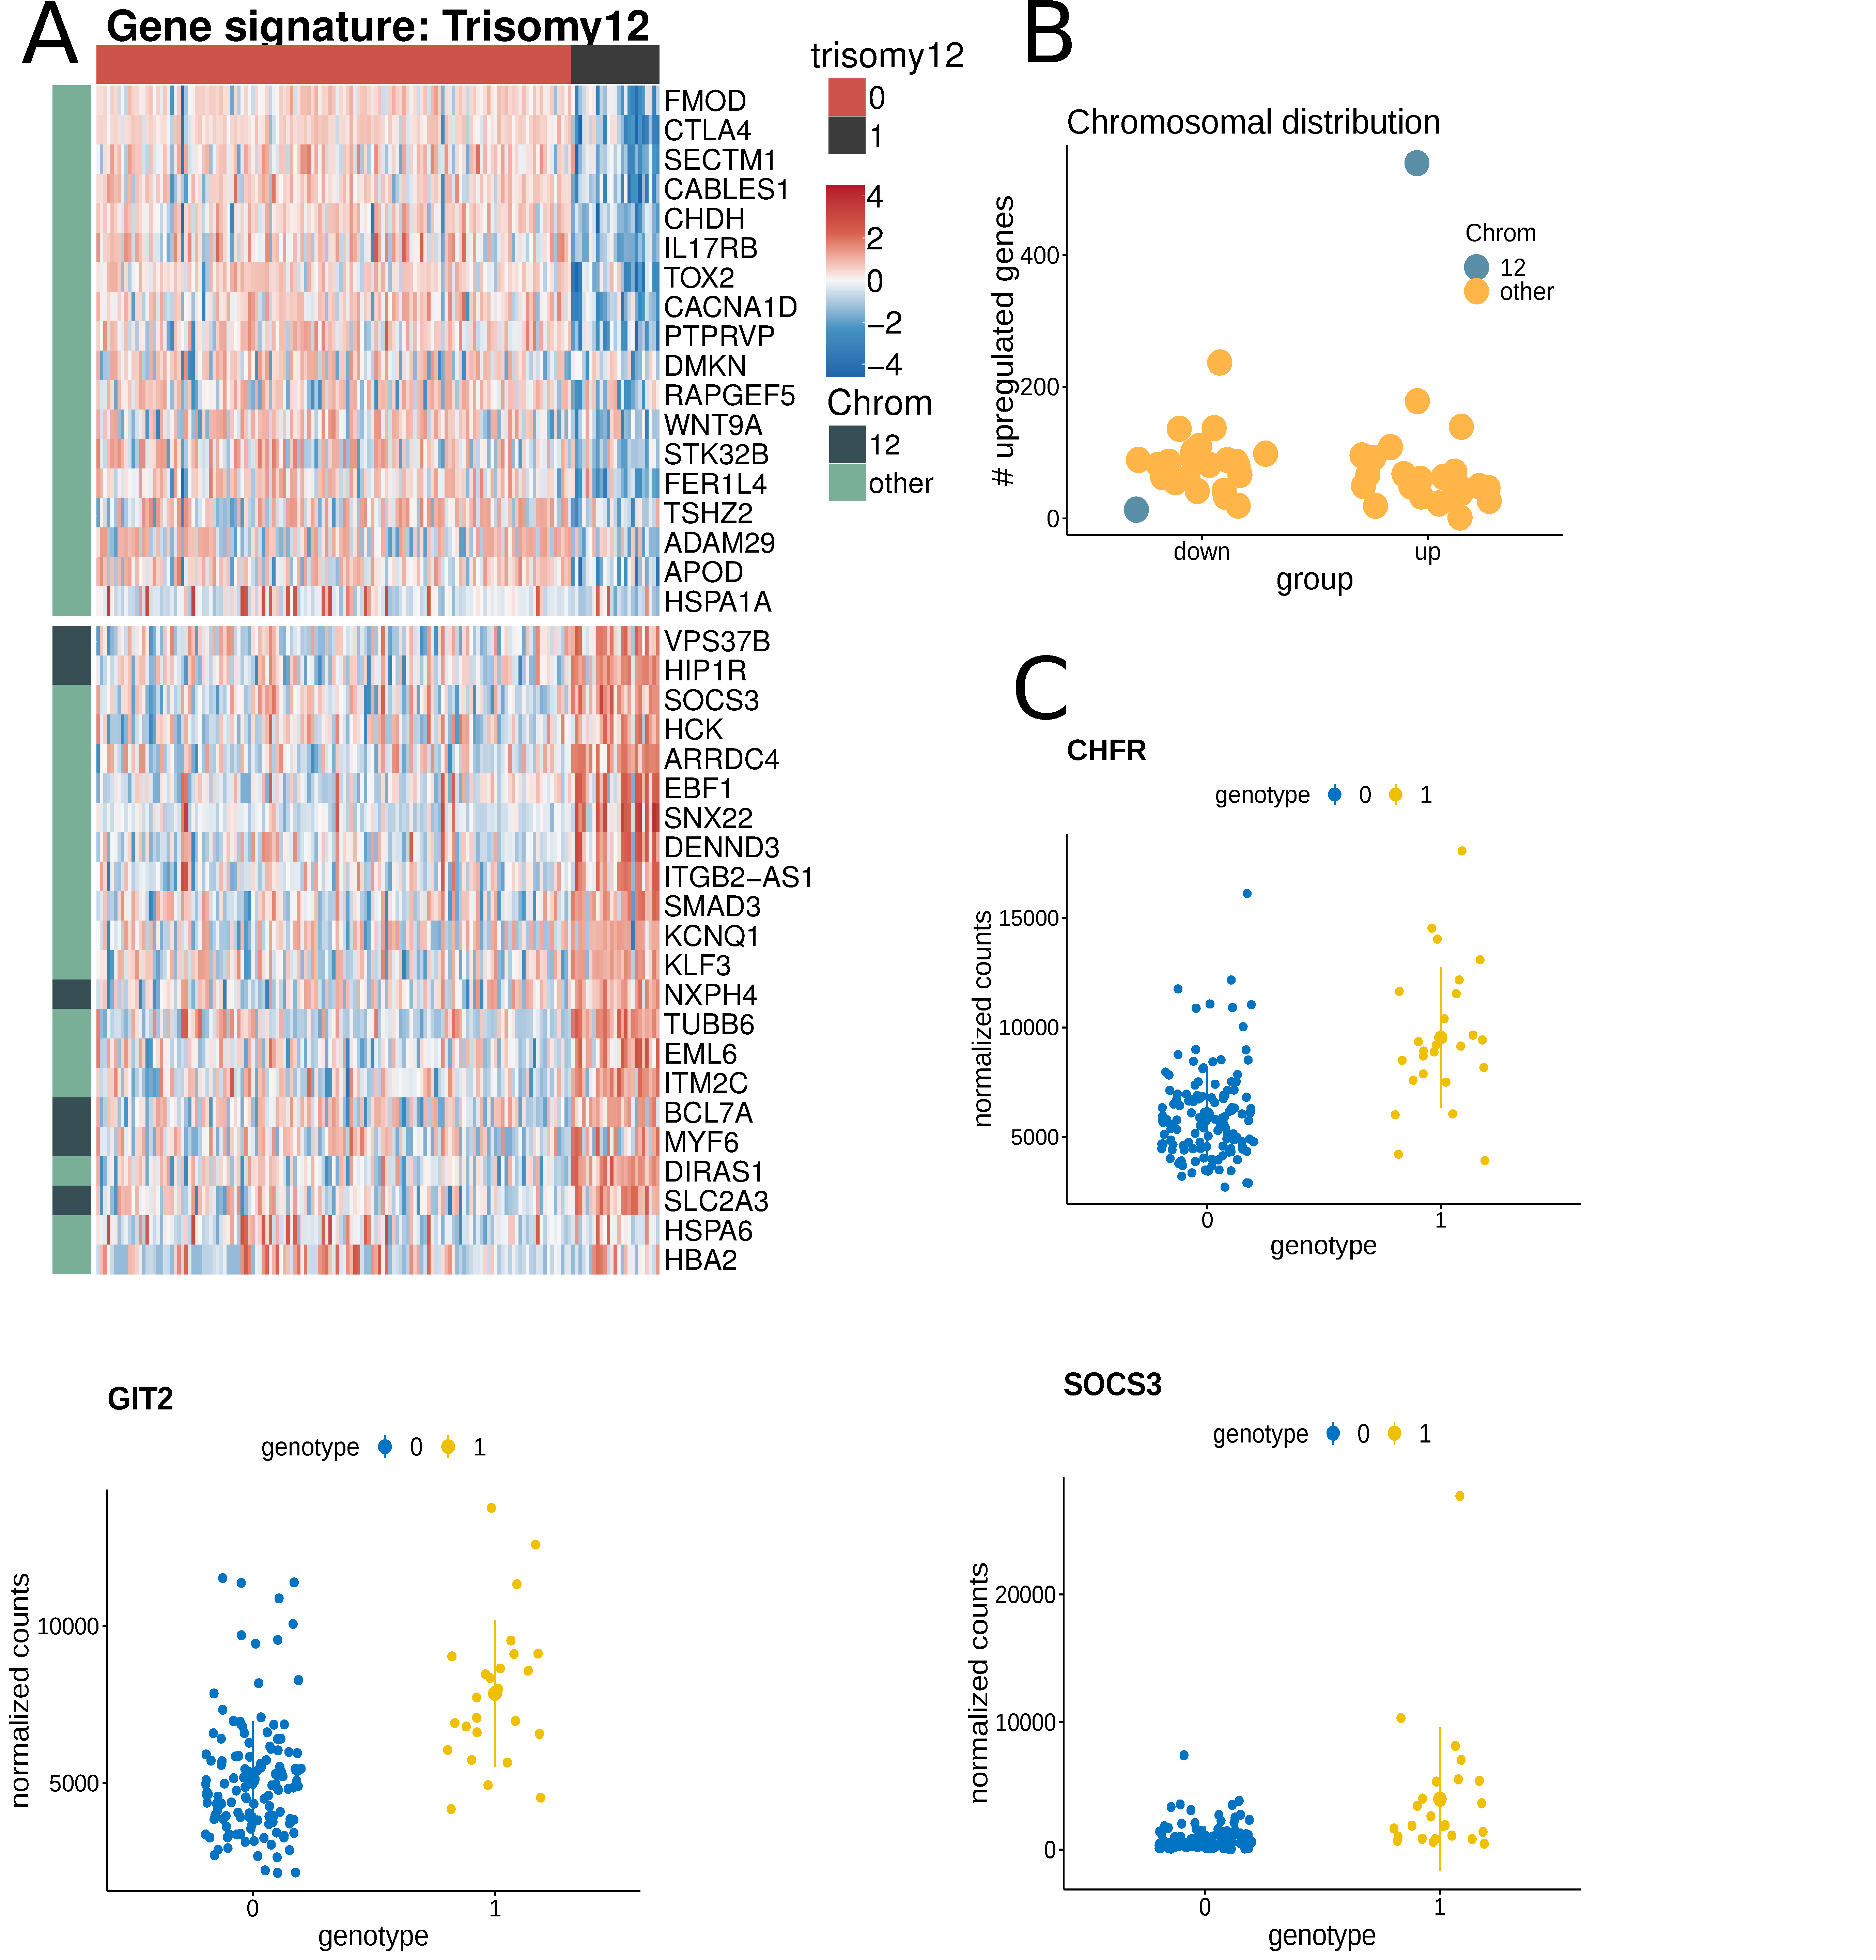
\includegraphics[width=\columnwidth]{figures/trisomy12_chromDist_genes.pdf}
	\caption{\textbf{Gene expression in Trisomy12:} A) Differentially expressed genes in Trisomy12 with $\text{p}_\text{adj} < 0.01$, $\log_2$ fold change $>2$ and basemean $> 500$. B) Role of dosage effect: Chromosomal distribution of differentially expressed genes in Trisomy12. Most upregulated genes are located on chromosome 12.} 
	\label{fig:trisomy12}
\end{figure}

\clearpage


\subsubsection{Other genomic driver of gene expression}
We also found numerous differentially expressed genes associated with other prevalent genetic variants (figure \ref {fig:data_overview}B). Mutation in the splicing factor SF3B1 gene showed more than 350 associations, indicating different layer of transcriptional aberrations within this variant. Among differentially expressed genes we found the chaperone gene UQCC. This gene has already been linked to SF3B1 mutations by differential isoform usage \citep{Reyes}. Here we show another layer of differential regulation and highlight its role. In addition, we were able to identify more than 100 differentially expressed genes in driver mutations such as BRAF and common CNVs as del17p13, del13q14 and del11q22.3 (figure \ref{fig:data_overview}B).
Top hits for each variant and enriched pathways of differentially expressed genes are shown in table \ref {tabular:summary}. We further evaluated the extend of a direct dosage effect from the chromosomal distribution within differentially expressed genes of CNVs. Deletions showed a similar degree of dosage related genes on downregulated genes as variants related to a gain on upregulated genes. But between variants the dosage effect varied (see figure \ref{fig:data_overview}B). In line with this the sizes of lesions vary between CNVs and even within sample with the same CNV.



\subsubsection{Intermediated programmed methylated samples form an independent cluster upon most variable genes.}
Based on methylation pattern, distinction by IGHV status was recently refined by introducing a categorization into low- (LP), intermediate- (IP), and high- (HP) programmed samples. As mutation status of IGHV, methylation pattern were associated with the maturation status of tumor precursor cells within haematopoietic cell lineage \citep{Oakes2016}. Using $t$-distributed stochastic neighbour embedding ($t$-SNE) we identified three cluster associated with these methylation groups based on the expression of the most variable genes (figure \ref {fig:data_overview}D). These findings confirm the relevance of methylation groups and a refined distinction of sample into these three groups to investigate CLL subtypes. Previous analysis of methylation pattern in CLL suggested a disease specific role of the transcription factors EGR, NFAT, AP1 and EGF by establishing aberrant methylation pattern \citep{Oakes2016}. In line with this, we found EGF1, NFAT and EGR1 among genes whose expression patterns are associated with methylation groups. 



\clearpage


\begin{table}
\begin{tabular}{ |p{1.6cm}|p{1cm}|>{\small}p{6.2cm}|p{7cm}| }
	\hline
	\multicolumn{4}{ |c| }{\textbf{Differentially expressed genes}} \\
	\hline
	\textbf{Variant} & \textbf{$\text{p}_\text{adj}$$<0.01$} & \textbf{Tophits} & \textbf{Kegg pathways} \\ \hline
	\multirow{4}{*}{trisomy12} & \multirow{4}{*}{3828} & ANAPC5, CHFR, LIX1, & Endocytosis, \\
	 && GIT2, ITFG2, ADD2, & Regulation of Actin Cytoskeleton,\\
	 && NCKAP1L, UACA, SCARB1 & Ubiquitin mediated proteolysis \\ \hline
	\multirow{4}{*}{IGHV} & \multirow{4}{*}{3557} & SLC16A9,NETO1,PLD1, & NK-cell mediated cytotoxicity, \\
	&& FRMD4B, PLEKHG4B,NPTX1, & Calcium signaling pathyway,\\
	&& KCNK9,PON1,PRR18, & Pathways in cancer\\ \hline
	\multirow{4}{*}{SF3B1} & \multirow{4}{*}{361} & APBB3,SRRM5,IFI27, & Melanogenesis,\\
	&& TFCP2L1,UQCC1,FBN1, & Cell cycle\\
	&& PSD2,FBLN2,HPCAL4 & Neuroactive ligand receptor interaction\\ \hline
	\multirow{4}{*}{del17p13} & \multirow{4}{*}{287} & CPT1C,NEURL4,MTTP, & Fatty acid metabolism, \\
	&& MTMR11,ZBTB4,SENP3, & Endocytosis,\\
	&& TFCP2L1,KIAA0753,RABEP1 & Cell cycle \\ \hline
	\multirow{4}{*}{BRAF} & \multirow{4}{*}{226} & TMPRSS3,SLC38A11,RAB25, & MAPK signaling pathway, \\
	&& DSP,	ARHGEF37,PAGE2B, & Hematopoietic cell lineage,\\
	&& RNF157,ZFHX4,KIF14,	& Wnt signaling pathway \\ 
	\hline
	\multirow{4}{*}{del11q22} & \multirow{4}{*}{171} & RNASE1, REXO2,USP28, & Cell cycle,\\
	&& CUL5,ATM, ALKBH8, & Ubiquitin mediated proteolysis,\\
	&& TMPRSS5,	NPAT,SIK2, & Pyruvate metabolism\\ \hline
	\multirow{4}{*}{del13q14} & \multirow{4}{*}{167} & ENPP3,TMPRSS4,CDCP1, & Pantheonate and COA biosyn., \\
	&& TSPAN13, RGL3,SLC1A6 & Starch and sucrose metabolism,\\
	&& INHBA,RAI14,SOAT2  & Riboflavin metabolism \\ \hline
	\multirow{4}{*}{TP53} & \multirow{4}{*}{95} & NOTCH4,PTPRB,MDM2	& Notch signaling pathway,\\
	 && TEAD1,TFCP2L1,CMYA5, & Adherens junction,\\
	 && LRRC63, MAP2K4, PAX9 & Dorso ventral axis form.\\ \hline 	 	 
	\multirow{4}{*}{Notch1} & \multirow{4}{*}{73} &  SPAG17,DSP,NOTCH4, & Antigen processing, \\
	&& GJB7,DNAH2,SH3RF1 & Spliceosome,\\
	&& POU6F2, ARHGEF37,SPACA9 & Huntingtons disease \\ 
	\hline
	\multirow{4}{*}{gain8q24} & \multirow{4}{*}{66} & LGSN,	ADGRG7,	CBS, & Selenoamino acid metab., \\
	&& SNTB1,E2F5,RAD21, & Glycine serine and threonine metab.,\\
	&& ZNF462,ZNF7,ADAMDEC1 & Cystein and metheonine metab. \\
	\hline	
	\multirow{4}{*}{del8p12} & \multirow{4}{*}{65} &  TRPM2-AS,PSPHP1,INTS9, & Basal cell carcinoma, \\
	&& MTCO3P12,LGSN,HMBOX1, & Hedgehog signaling pathway,\\
	&& KIF13B, LINC01016, FERMT2 & Alzheimers disease \\ 
	\hline
	\multirow{4}{*}{MED12} & \multirow{4}{*}{35} &  CDH20,LGSN,CSPG5,& Lysosome, \\
	&& MYO5C, ERRFI1,ADGRG7, & Intest. immune network for IGA prod.,\\
	&& FCRL4,CLCNKA,KLF4 & Neurotrophin signaling pathway \\ 
	\hline
	\multirow{4}{*}{ATM} & \multirow{4}{*}{24} &  RNASE1,SNTB1,PPM1E,  & Gap junction, \\
	&& RBFOX2,SAXO2,PLCB1,  & Vascular smooth muscle contr.,\\
	&& CYP51A1-AS1,CAMK2A,P4HA2 & Phosphatidylinositol sig. system \\ 
	\hline
\end{tabular}
\caption{\textbf{Summary differentially expressed genes in genomic variants}: Number of differentially expressed genes, tophits and top enriched pathways are shown.}
\label{tabular:summary}
\end{table}

\clearpage


\subsection{ IGHV status and Trisomy12 interact in an epistatic way determining gene expression}

Most CLL samples show high mutational burden with around 2000 molecular lesions in the entire tumour genome \citep{Gaidano2017}. Even though most of them are rather related to genomic instability than being functional or tumour driving events, CLL is still characterized by an interplay of numerous genetic changes and environmental factors. In our cohort CLL samples carry about 3 of the tested variants on average (see Supplement figure \ref{fig:mutation_overview}A). To investigate the role of genetic interaction we tested their collaborative effect on gene expression phenotypes. We investigated the epistatic gene expression changes in the most severe genomic alterations the IGHV status and Trisomy12. Epistasis was defined as a non-linear effect on gene expression between sample with both variants co-occuring and the single variants alone \citep{Fisher1919}. \\

In total 893 genes showed specific expression pattern in a combined genotype  
($\text{p}_\text{adj} < 0.1$). These expression changes differed from the expected change by simple combination of the single variant's effects. We observed different ways of epistatic interaction and clustered genes by them (see figure \ref{fig:mixed_epistasis}A). We distinguished between the following types of mixed epistasis (see figure \ref{fig:mixed_epistasis}B): Buffering, when the up or downregulation of a gene by a genetic variant was strongly enhanced in sample with the combined genotype. Inversion, when the effects in the single variants alone were reversed in the combined genotype. Suppression, when a strong up or downregulation of a gene in one or both variants alone was absent in samples with both variants. 
In total we identified five cluster of genes representing different ways of mixed epistasis as inversion down, suppression, different degrees of buffering and inversion up (see figure \ref{fig:mixed_epistasis}A from top to bottom). Different types of epistasis are also shown on the level of gene counts of single genes at the example of the adhesion mediating protein coding gene CHAD (inversion), the endonuclease encoding gene GEN1 (buffering up) and the transcription factor LEF1 (suppression)(see figure \ref{fig:mixed_epistasis}C). \\

These findings strongly suggest a functional association between the IGHV status and trisomy12 in CLL. The IGHV hypermutation status characterizes the B cell receptor signalling activity. This seem to impact trisomy12 related mechanisms as well. To further investigate this interaction we used enrichment tests for genes in the different mixed epistasis cluster. We found genes upregulated in trisomy12 U-CLL sample, but suppressed in M-CLL trisomy12 samples were enriched in Wnt beta catenin and Notch signaling.
Notch signaling has shown to synergize with B cell receptor signalling before \citep{Thomas2007}. Besides this, regulation of integrins in trisomy12 samples is modulated by notch signalling \citep{Riches2014}. This suggests decreased B cell receptor activity in M-CLL sample effect trisomy12 depended integrin expression via notch signalling. 
In contrast genes in other cluster as those showing a strong buffering effect were enriched in G2M checkpoint pathway. This points towards changes in cell cycle mechanisms as an alternative tumour driver (see figure \ref{fig:GSEA_hallmark}). 

\subsection{The interaction between IGHV status and trisomy12 affect \textit{ex vivo} drug response in CLL}

Ex vivo sensitivity to drugs is an informative cellular phenotype that reflects pathway dependencies of the tumor cells. We therefore asked whether the epistatic interaction between IGHV status and trisomy12 on expression level also affects the drug response phenotype.  In our previous PACE project, we measured the the ex vivo sensitivity of 184 CLL samples towards 63 compounds \citep{Dietrich}. Using the same epistasis model on the drug screening dataset from PACE, we identified 6 drugs whose effect on cell viability was significantly affected by the interaction between IGHV and trisomy12 (see figure \ref{fig:drugEpistasis-1}) ($\text{p}_\text{adj} < 0.1$). For four drugs, namely, vorinostat, NU7441, fludarabine and AZD7762, we observed a suppression effect of the trisomy12 phenotype by IGHV status: compared with non-trisomy12 samples, the trisomy12-only samples showed increased sensitivity to those four drugs, indicated by the lower viability of cells after drug treatment. Additional presence of IGHV mutation reduced sensitivity to those four drugs. While for the other two drugs, chaetoglobosin A and BIX02188, the samples with combined IGHV mutation and trisomy12 showed increased resistance compared with either wild type samples, IGHV mutated samples or trisomy12 samples. 

%Interestingly, all of the four drugs that show the "supression of trisomy12" phenotype directly or indirectly target DNA: NU7441 inhibits DNA-dependent protein kinase (DNA-PK) and therefore potentiate DNA double-strand breaks \citep{Leahy2004, Zhou2017}, AZD7762 is a checkpoint kinase (CHEK) inhibitor, which can impare DNA repair and increases cell death \citep{Zabludoff2008}, fludarabine directly inhibits DNA synthesis and disrupt cell cycle \citep{Ricci2009}, vorinostat, a histone deacetylase (HDAC) inhibitor, was also reported to induced Reactive Oxygen Species and DNA damage in leukemia cells \citep{Petruccelli2011}. As mentioned above, we observed a enrichment of the genes showing strong buffering effect in the G2M checkpoint pathway, indicating compared with trisomy12-only samples, the samples with both trisomy12 and IGHV mutation have more functional DNA damage checkpoint machinery and therefore they are more resilient to the disruption of DNA damage response. 
Overall, the interaction of IGHV mutation and trisomy12 on drug response phenotype level further validates the presence of the epistasis effect of IGHV and trisomy12 in CLL and implicates this effect is functional relevant and maybe further explored for clinical therapeutics. 
\clearpage


\begin{figure}
  \centering
  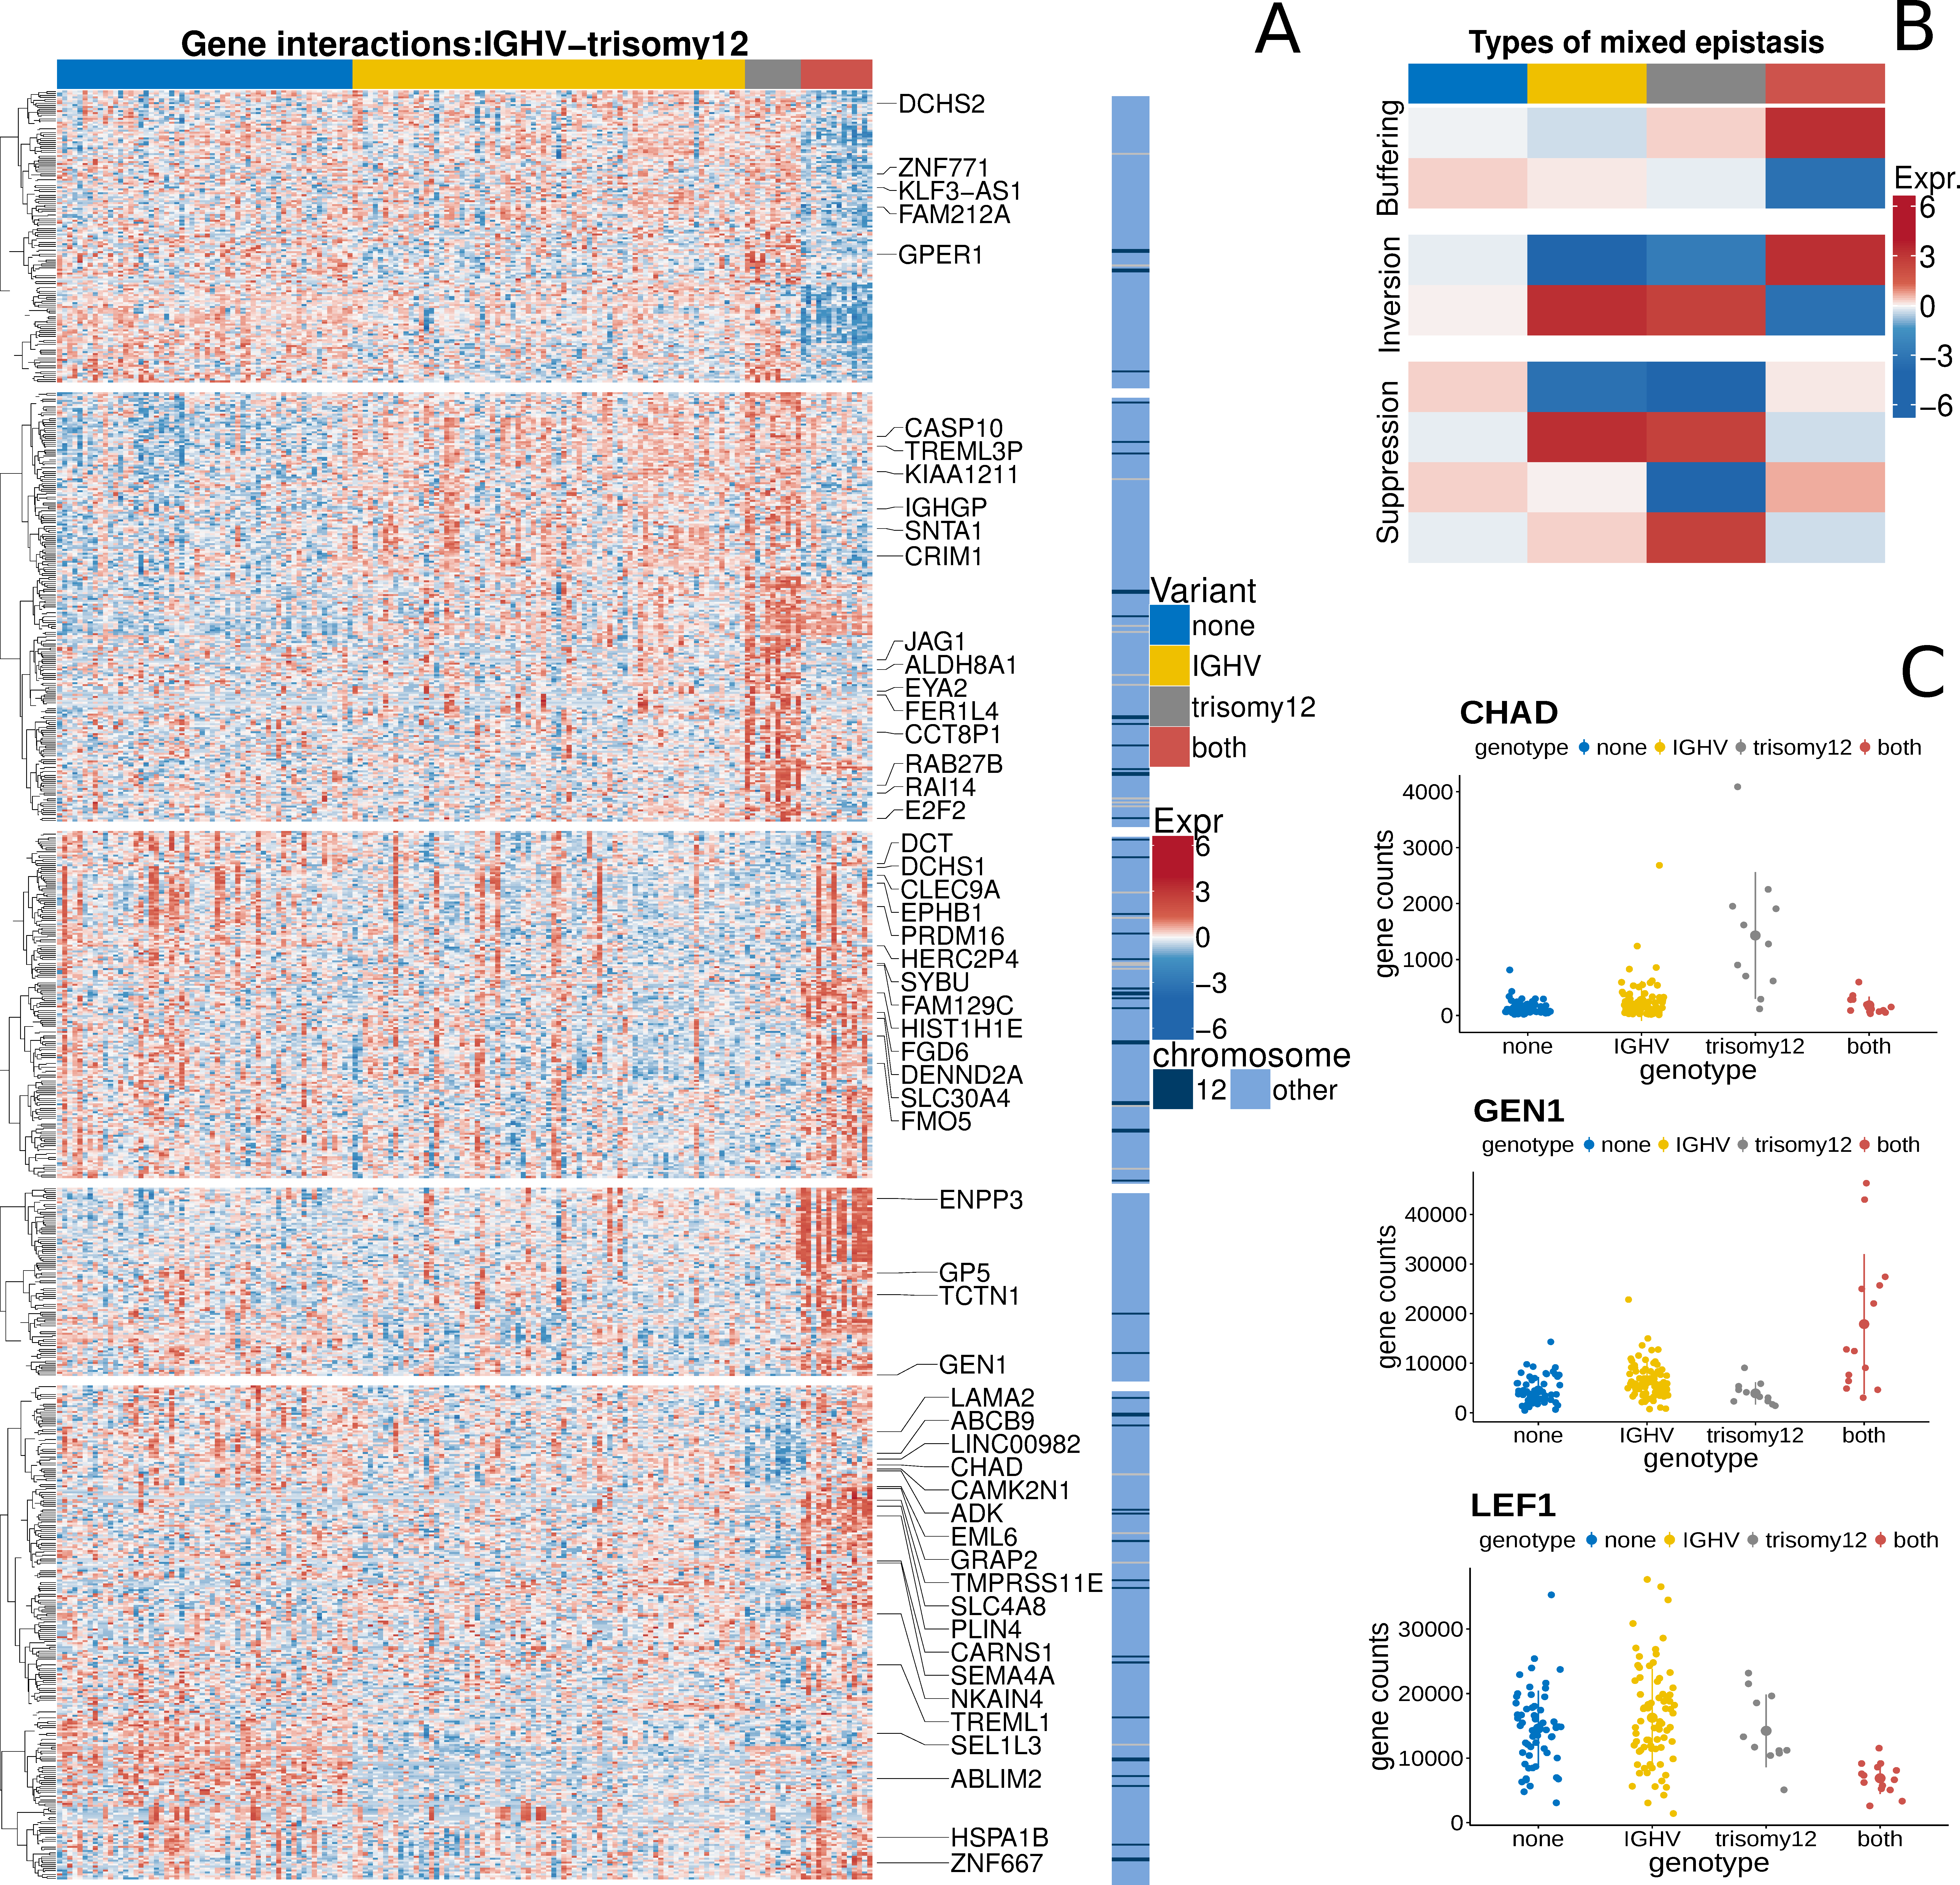
\includegraphics[width=\columnwidth]{epistasis_Deseq_general.pdf}
  \caption{\textbf{Mixed epistasis in Trisomy12 and IGHV mutated samples:} A) Expression of epistatic gene interactions between Trisomy12 and M-CLL ($\text{p}_\text{adj} < 0.1$). Genes are clustered by different ways of epistatic interaction. B) Scheme of mixed epistasis in CLL samples: buffering, inversion, suppression. C) Epistatic expression of single genes. Raw gene counts of CHAD ($\text{p}_\text{adj} = 6.17\times10^{-08}$), GEN1 ($\text{p}_\text{adj} = 1.47\times10^{-04}$) and LEF1 ($\text{p}_\text{adj} = 6.21\times10^{-03}$) show different ways of epistasis as supression, buffering up and buffering down.}
  \label{fig:mixed_epistasis}
\end{figure}

\clearpage

%\begin{figure}
%	\centering
%	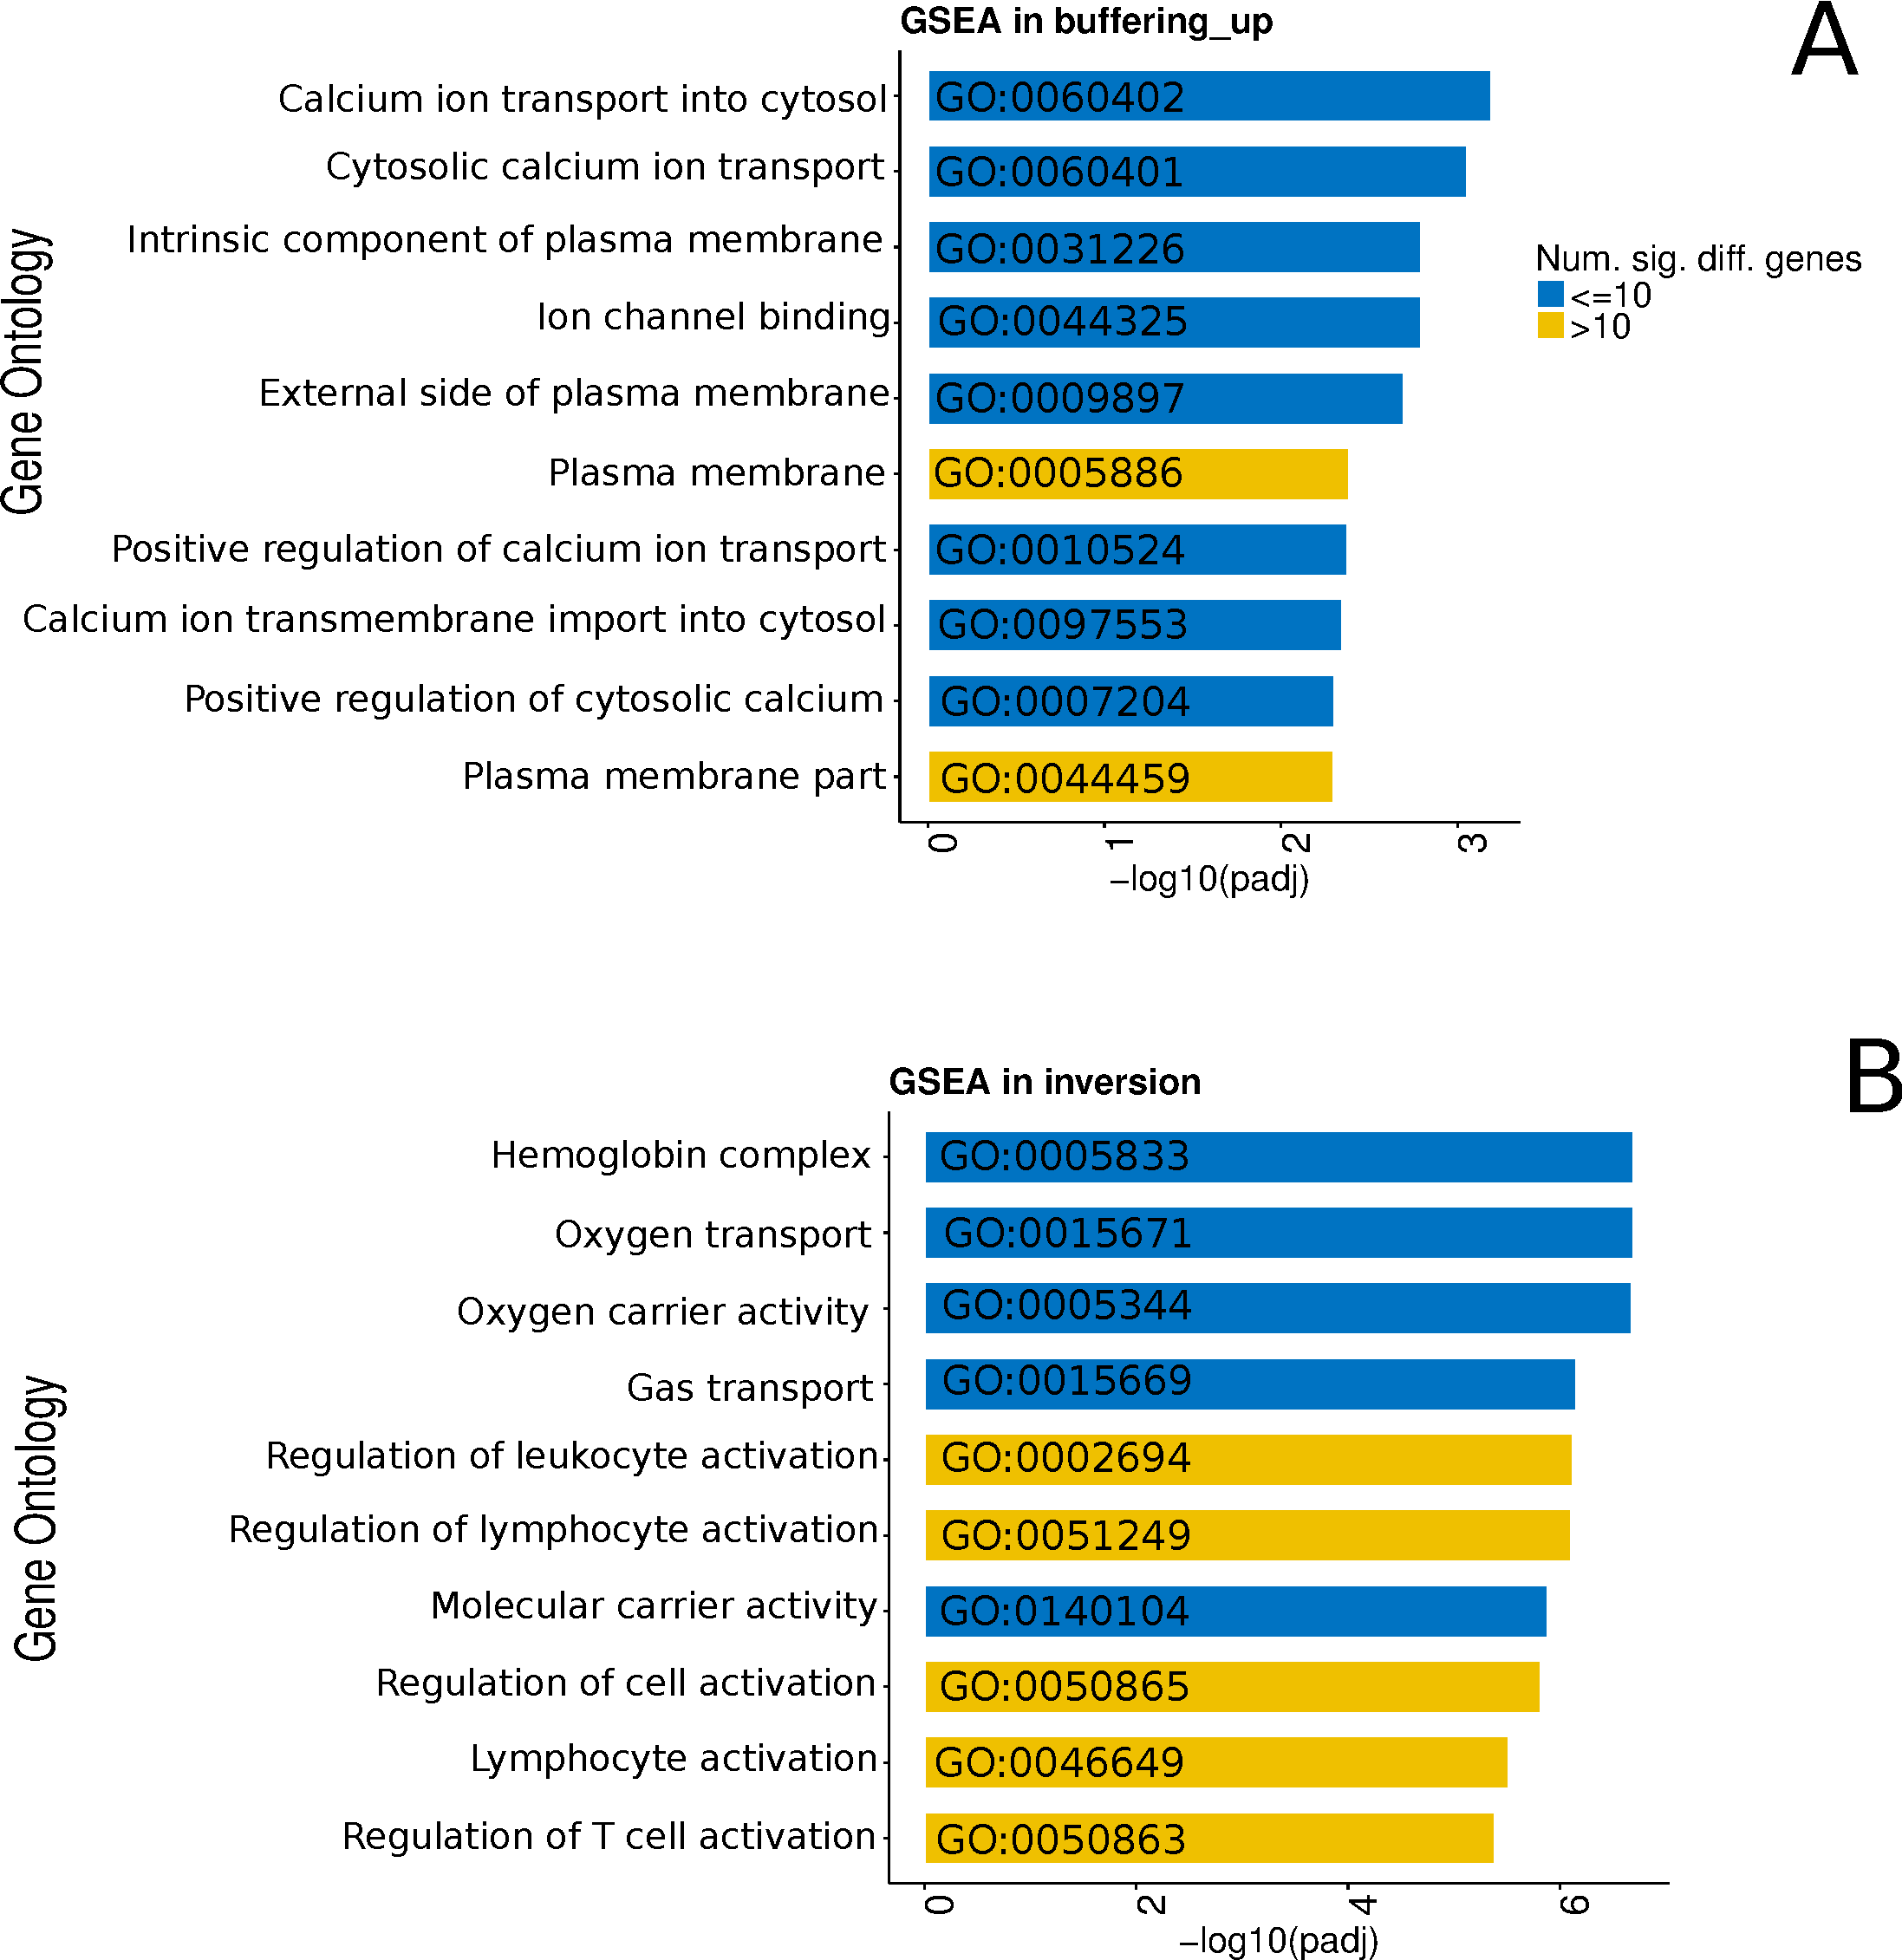
\includegraphics[width=\columnwidth]{enrichment/GSEA_combined.pdf}
%	\caption{\textbf{Gene set enrichment analysis of mixed epistasis cluster:} A) Genes showing a strong positive buffering effect are upregulated in pathways related to calcium transport and regulation B) Genes which show an inversion effect are enriched in pathways related to lymphocyte and leukocyte activation.}
%	\label{fig:GSEA}
%\end{figure}



\clearpage

\begin{figure}
	\centering
	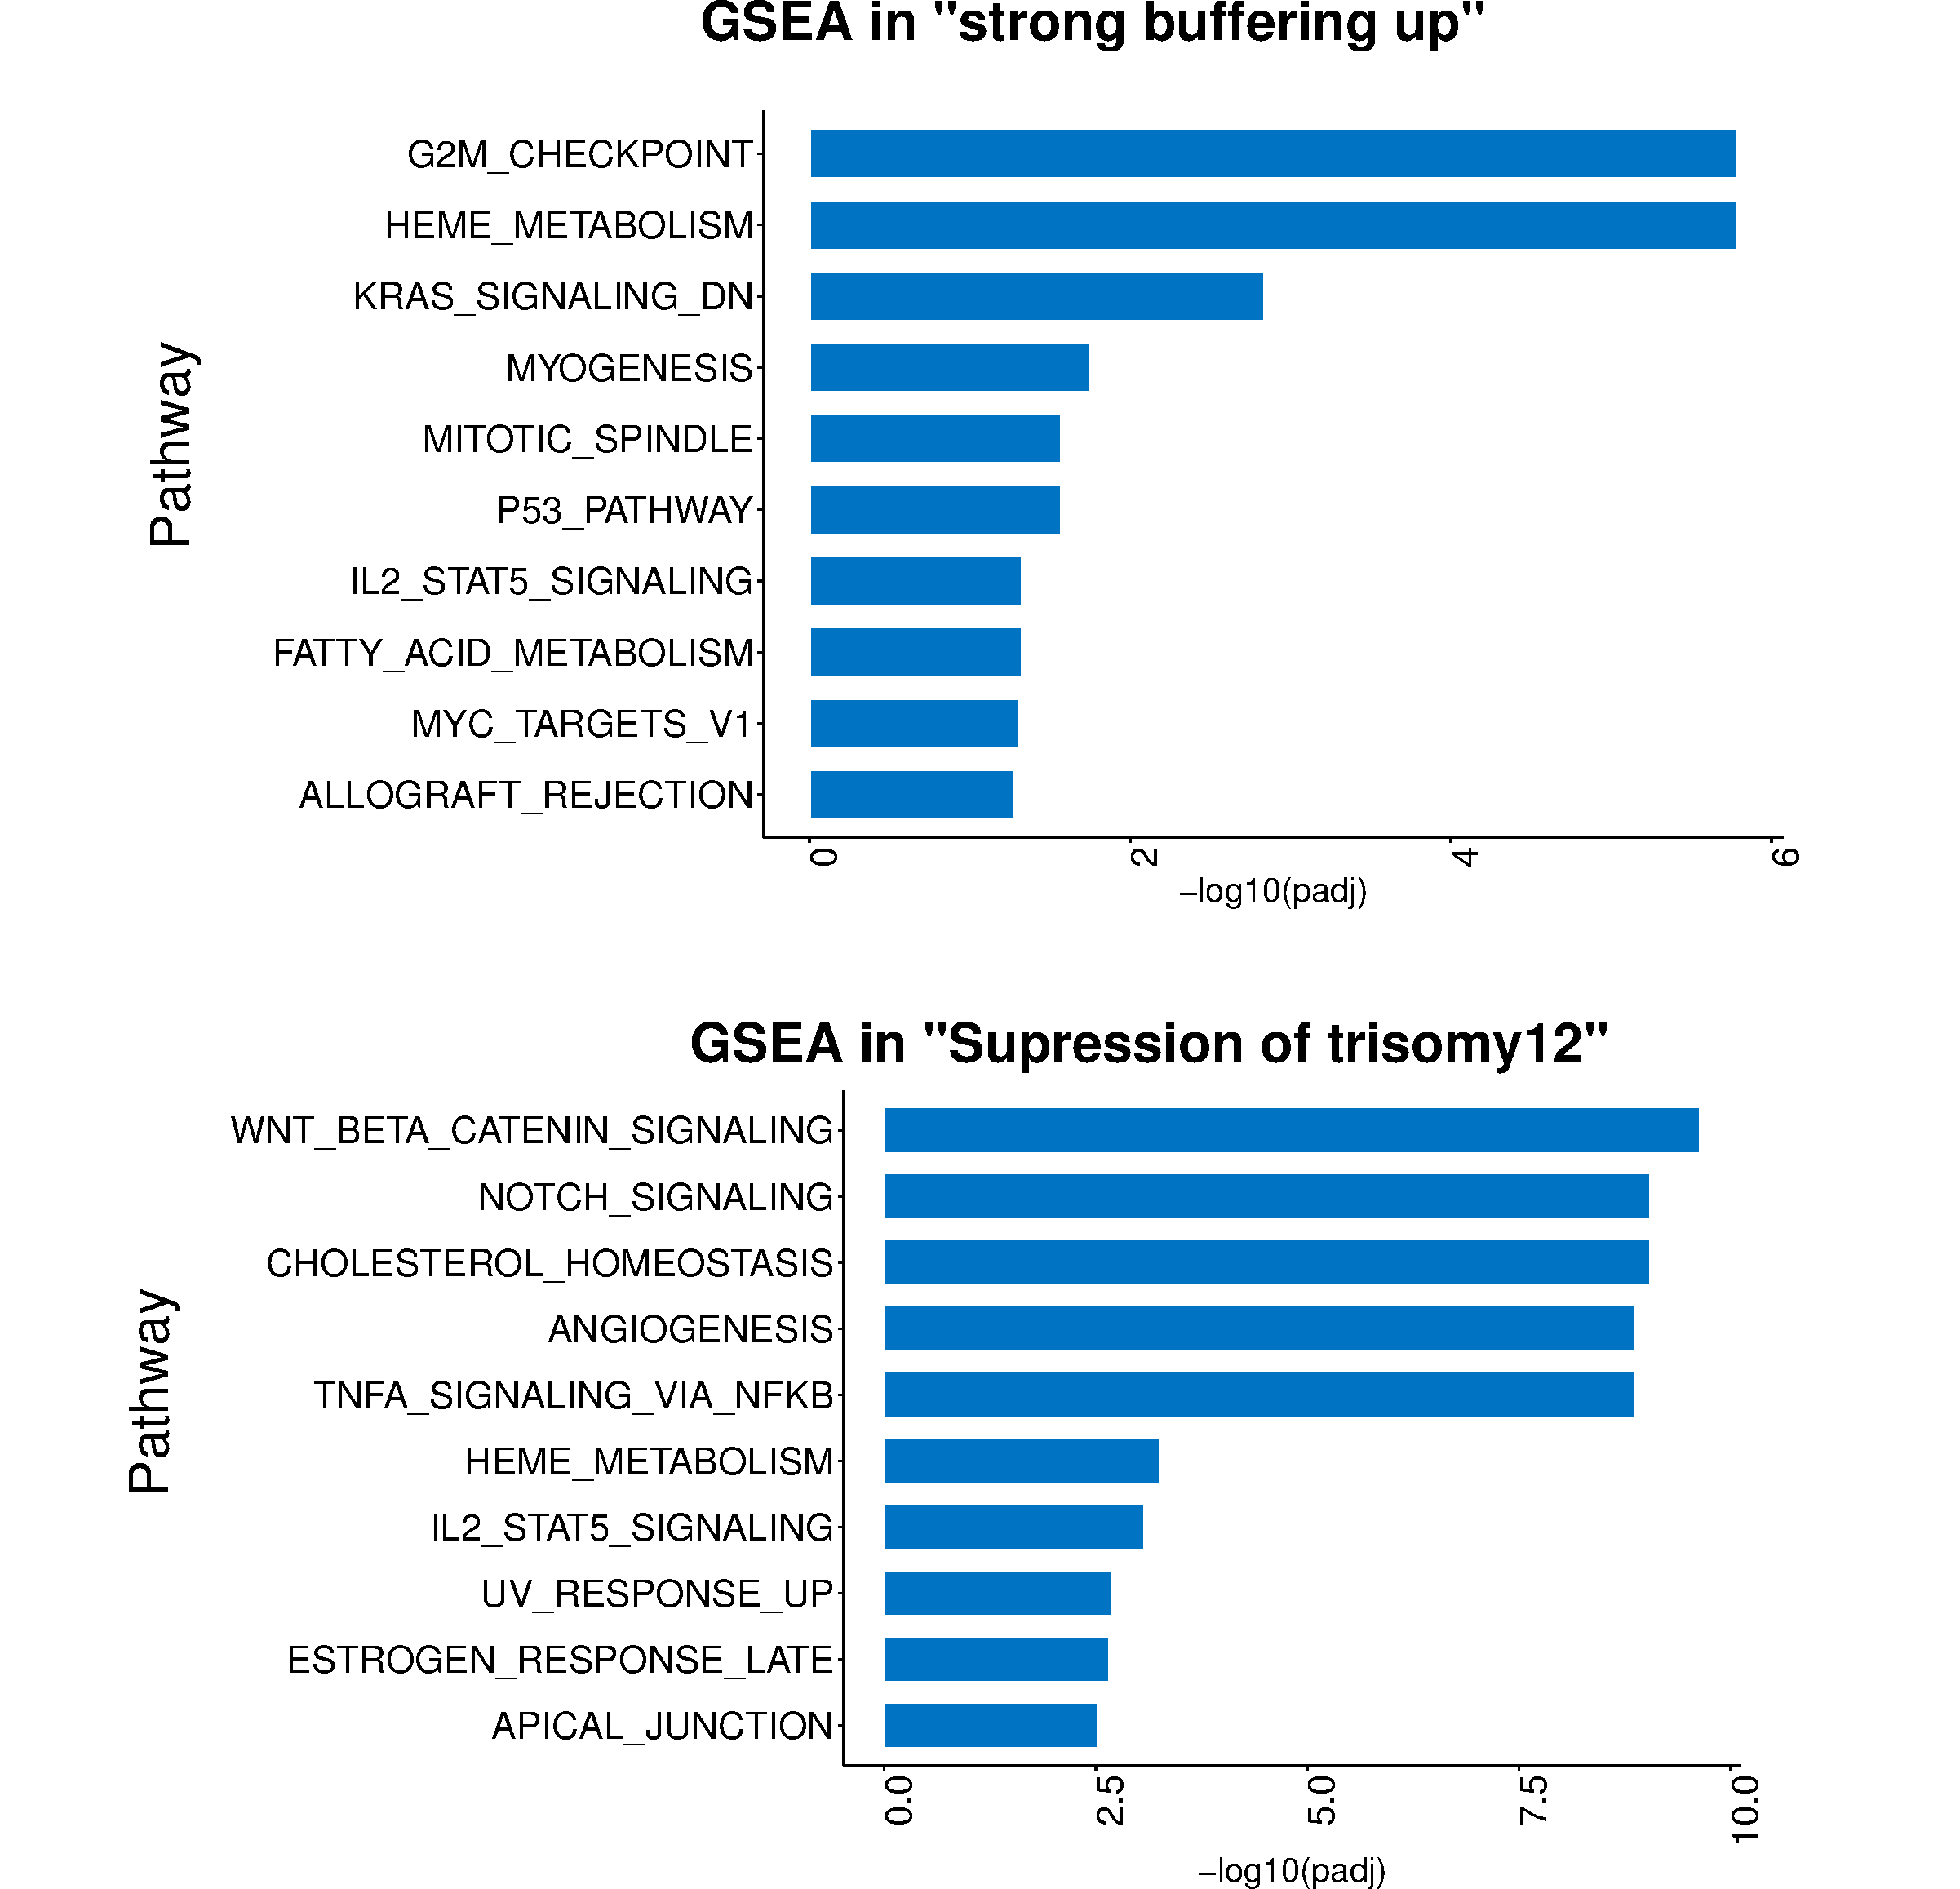
\includegraphics[width=\columnwidth]{GSEA_Hallmark.pdf}
	\caption{\textbf{Gene set enrichment analysis of mixed epistasis cluster:} A) Genes showing a strong positive buffering effect are upregulated in pathways related to G2M checkpoint genes and heme metabolism B) Genes which show an suppression compared to Trisomy12 only samples are enriched in pathways related to Notch signaling pathway and Wnt-beta-Catenin signaling}
	\label{fig:GSEA_hallmark}
\end{figure}


\clearpage

\begin{figure}
	\centering
	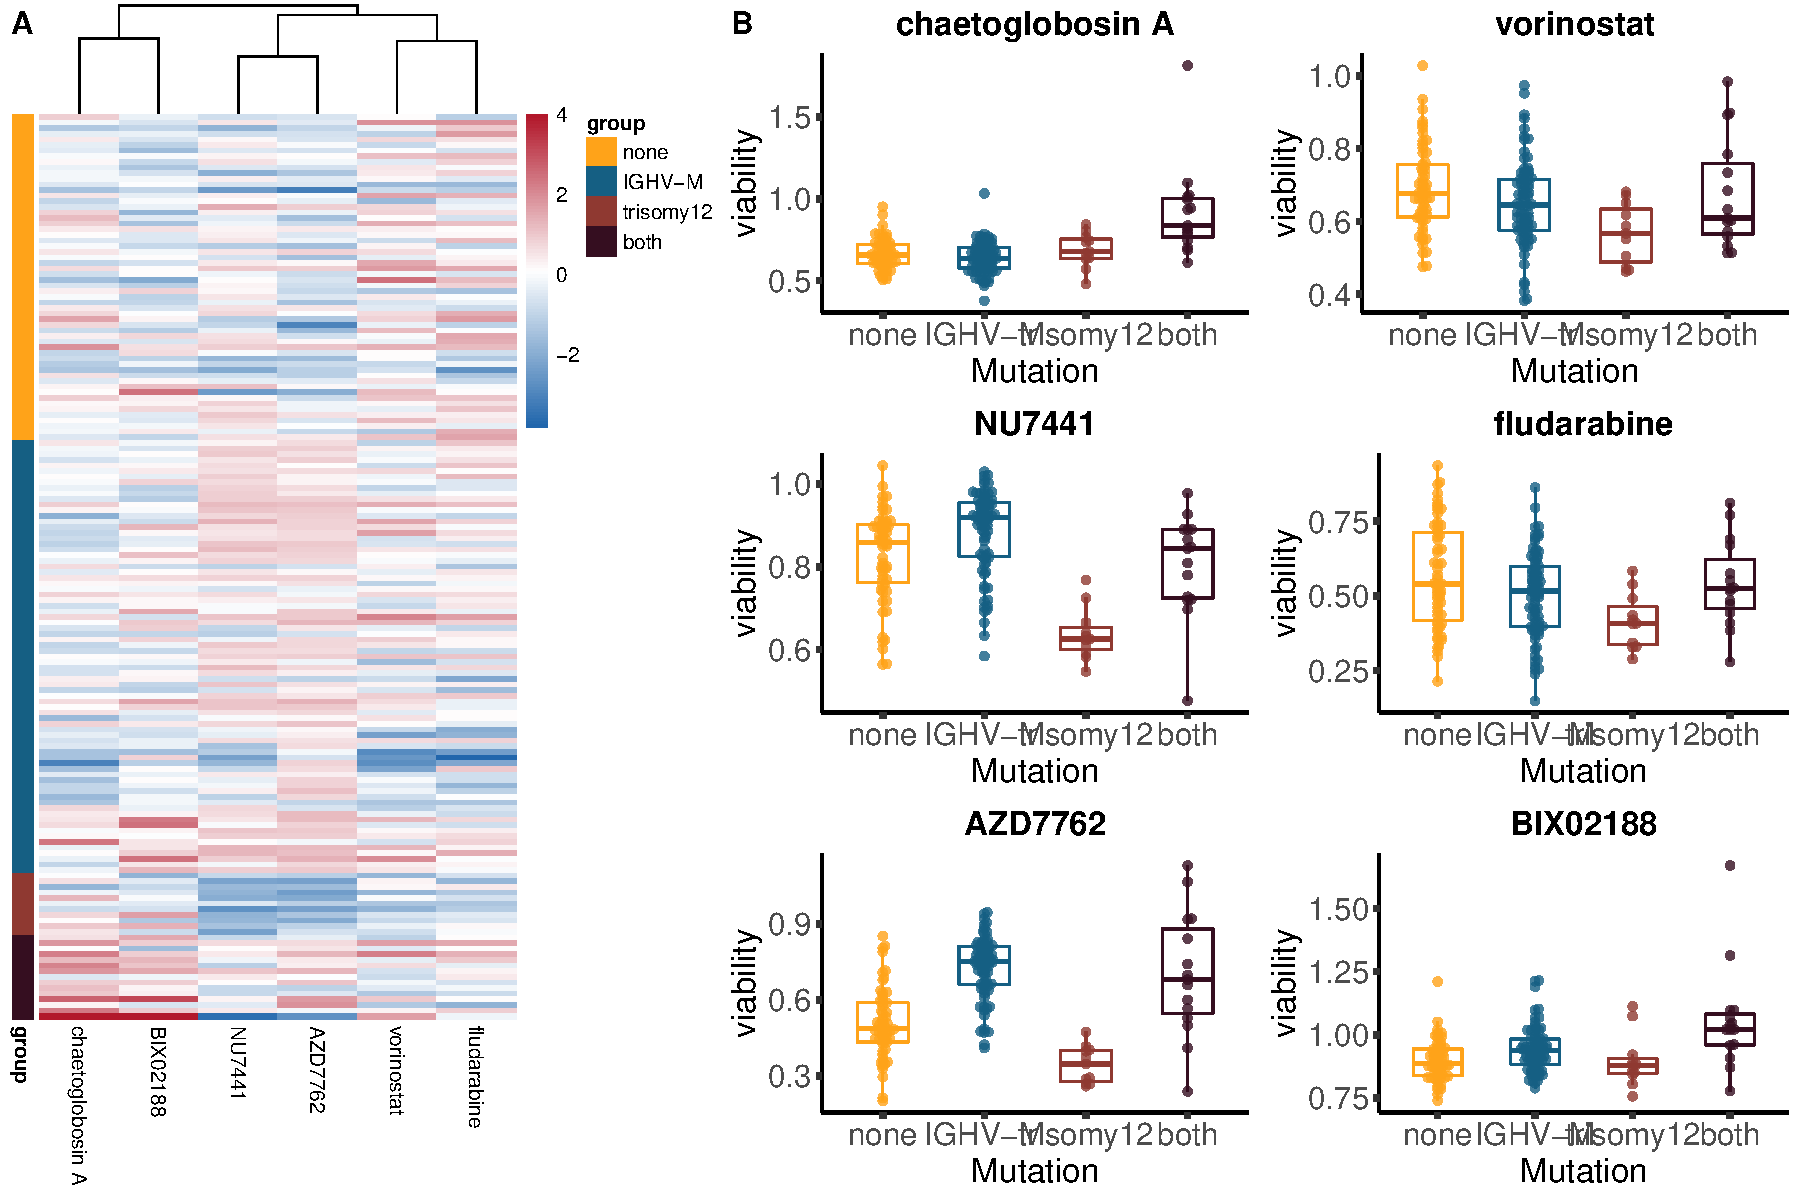
\includegraphics[width=\columnwidth]{drugEpistasis-1.pdf}
	\caption{\textbf{Gene set enrichment analysis of mixed epistasis cluster:} A) Genes showing a strong positive buffering effect are upregulated in pathways related to G2M checkpoint genes and heme metabolism B) Genes which show an suppression compared to Trisomy12 only samples are enriched in pathways related to Notch signaling pathway and Wnt-beta-Catenin signaling}
	\label{fig:drugEpistasis-1}
\end{figure}